\documentclass[11pt,a4paper,xcolor=dvipsnames]{beamer}
\usetheme{Berlin}
\usepackage[latin1]{inputenc}
\usepackage[english]{babel}
\usepackage{graphicx}

\usepackage{lmodern}

\author[Michael Cabot \and Sander Latour]{Michael Cabot \and Sander Latour}
\institute{University of Amsterdam}
\title[iMSG]{iterative Minimal Semantics Grammar [iMSG]}

\date{21 maart 2013}

\begin{document}

\begin{frame}
\titlepage
\end{frame}

\begin{frame}
\tableofcontents
\end{frame}

\section{Contribution}
\begin{frame}
  \begin{center}
    \textit{How the poverty of the stimulus solves the poverty of the stimulus}\\
    \vfill
    \textbf{combined with}\\
    \vfill
    \textit{The Negotiation and Acquisition of Recursion Grammars as a Result of Competition Among Exemplars}
  \end{center}
\end{frame}

\begin{frame}
  \begin{center}
    \textit{Iteratively evolve a grammar to make it more learnable}\\
    \vfill
    \textbf{combined with}\\
    \vfill
    \textit{Learning a semantic grammar from observations}
  \end{center}
\end{frame}

\begin{frame}
  \begin{center}
    \textit{Iteratively evolve a grammar to make it more learnable}\\
    \vfill
    \textbf{Iteratively evolve a semantic grammar}\\
    \vfill
    \textit{Learning a semantic grammar from observations}
  \end{center}
\end{frame}

\section{Motivation}
\begin{frame}
  \begin{itemize}
    \item \hspace*{0pt}[Zuidema2003] needed to force minimal language size
    \item Language is driven by the need to communicate semantic messages
    \item The necessity to be able to communicate may make forcing obsolete
    \item The negotiation model of [Batali1999] seems convertable to the iterative process of evolution
  \end{itemize}
\end{frame}

\section{Iterative Learning}
\begin{frame}
  \begin{center}
    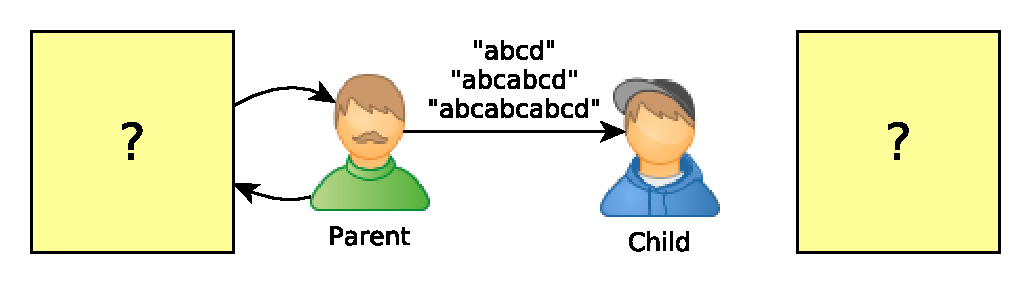
\includegraphics[scale=0.6]{assets/iterative1.pdf}
  \end{center}
\end{frame}

\begin{frame}
  \begin{center}
    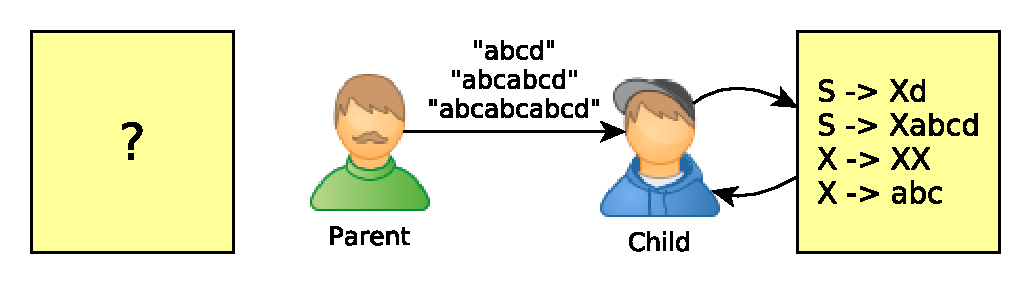
\includegraphics[scale=0.6]{assets/iterative2.pdf}
  \end{center}
\end{frame}

\begin{frame}
  \begin{center}
    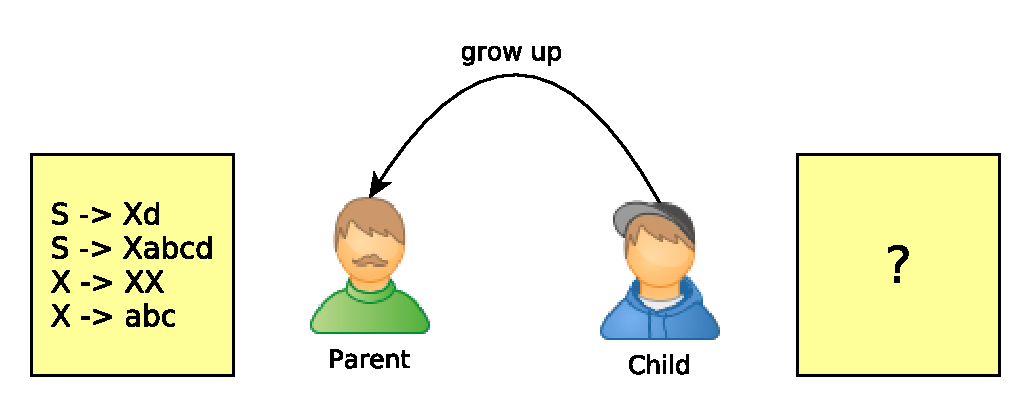
\includegraphics[scale=0.6]{assets/iterative3.pdf}
  \end{center}
\end{frame}

\section{Working with semantics}
\begin{frame}
  Summary of batali (recap) (Sander)
Intuition behind learning from observations
small example of a few generated observations and a derived model
  encourage / discourage
\end{frame}

\begin{frame}{Vocabulair}
  \begin{columns}[c]
    \column{.65\textwidth}
      \begin{description}
        \item[meaning] set of predicates and relations
        \item[sentence] tuple of strings (i.e. words)
        \item[observation] Alignment of meaning and sentence
        \item[phrase] Hierarchical structure linking meaning to a composition of strings
      \end{description}
    \column{.35\textwidth}
      \includegraphics[scale=0.2]{assets/examplar514a.png}
  \end{columns}
  \hfill \includegraphics[scale=0.2]{assets/observation514.png}
\end{frame}

\section{iMSG Components}
\begin{frame}
  Generating observations (Michael)
\end{frame}

\begin{frame}
  ViterbiX (short description of the extension) (Michael)
\end{frame}

\begin{frame}
  Learning from observations using viterbix (Michael)
\end{frame}

\begin{frame}
  Evaluation (Michael)
\end{frame}

\section{Status}
\begin{frame}
  Current state / Future plans (Sander)
\end{frame}
\end{document}
